\documentclass[12pt]{article}
% REVISION NOTES %%%%%%%%%%%%%%%%%%%%%%%%%%%%%%%%%%%%%%%%%%%%
% 2008-0814 Location, Date, Time
% 2008-0814 fixed citations -- added bibliography.
%
%
\usepackage{geometry}                
\geometry{letterpaper}                   
%\geometry{landscape}                
\usepackage[parfill]{parskip}    
\usepackage{daves,fancyhdr,natbib,graphicx,dcolumn,amsmath,lastpage,url}
\usepackage{amsmath,amssymb,epstopdf,longtable}
\usepackage[final]{pdfpages}
\DeclareGraphicsRule{.tif}{png}{.png}{`convert #1 `dirname #1`/`basename #1 .tif`.png}
\pagestyle{fancy}
\lhead{CE 3305 -- Fluid Mechanics -- SPRING 2024}
\rhead{Name:\_\_\_\_\_\_\_\_\_\_\_\_\_\_\_\_\_\_\_\_\_\_\_\_\_\_\_\_\_\_\_\_\_\_\_\_\_\_\_\_\_\_\_\_}
\lfoot{CE 3305 -- Cleveland}
\cfoot{Page \thepage\ of \pageref{LastPage}}
\rfoot{REVISED: ~4 FEB 2024}
\renewcommand\headrulewidth{0pt}
%%%%%%%%%%%%%%%%%%%%%%%%%%%%%%%%%%%%%%%%%%%%%%%%%%%%%%%
\begin{document}
\section*{\center{ { CE 3305 -- Fluid Mechanics} {Exam 1} } }
\section*{Purpose}
Demonstrate ability to apply fluid mechanics and \textbf{problem solving principles} covering topics such as: Fluid properties, viscosity, vapor pressure, fluid statics and pressure.
\section*{Instructions}
\begin{enumerate}
\item Put your name on each sheet you submit.  
\item Use additional sheets as needed. 
\item Begin each problem on a separate page.  Ok to disassemble to keep pages in order.
\item Do not write on the back of sheets (I won't look)
\item Use the problem solving protocol in the class notes.  The discussion sections can simply be the word ``discussion'' 
\item Label and/or underline answers, be sure to include units.
\end{enumerate}
\section*{Allowed Resources}
\begin{enumerate}
\item Your notes
\item Your textbook
\item The mighty Internet with following proviso
\item  \textbf{You may not communicate with other people during the exam}
\end{enumerate}
\noindent\rule{\linewidth}{0.4pt}
\clearpage

\begin{enumerate}
\item Argon gas is used as a sheilding gas for welding for fabrication of metal objects. A 200-liter tank has an empty mass of 50 kg. \\ \\
Determine:
\begin{enumerate}
\item The total weight of the 200-liter tank of argon at a pressure of 3,500 psia at a temperature of 313$^o$K.  
\item The argon pressure if the tank is submersed in the North Sea to repair an underwater pipeline, where the ambient water temperature is 6$^o$C
\item The additional ballast (mass) required for the tank to be neutrally bouyant in seawater ($\rho_{sw}= 1025 \frac{kg}{m^3}$)
\end{enumerate}
\noindent\rule{\linewidth}{0.4pt}
\clearpage
%~\newline
%\clearpage
%\item A fixed mass of water has a bulk modulus of compressibility of $2.2 \times 10^{9} ~Pa$. \\ \\
%Determine:
%\begin{enumerate}
%\item The pressure increase ($\Delta p$) required to reduce the volume of a mass of water by 2-percent (2 \%)
%\end{enumerate}
%\noindent\rule{\linewidth}{0.4pt}
%\clearpage
%\noindent\rule{\linewidth}{0.4pt}
\item The figure below is a schematic of a sliding plate viscometer used to measure the viscosity of a fluid. The top plate is moving to the right with a constant velocity in response to a force of 3 Newtons.
 

\begin{figure}[htbp] %  figure placement: here, top, bottom, or page
   \centering
   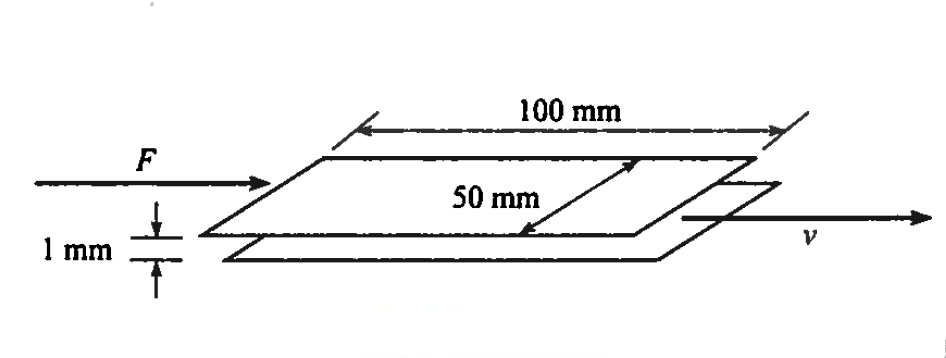
\includegraphics[width=4in]{SlidingPlateViscosity.png} 
   \caption{}
   \label{fig:slidingplateviscosity}
\end{figure}

Determine:
\begin{enumerate}
\item The speed of the plate if the viscosity is $\mu=5 \times 10^{-2}~\frac{N \cdot s}{m^2}$
\item The speed of the plate if the viscosity is $\mu=7 \times 10^{-2}~\frac{N \cdot s}{m^2}$
\item The viscosity if the speed of the plate is 10.001 $\frac{m}{s}$
\end{enumerate}
\noindent\rule{\linewidth}{0.4pt}
%\clearpage
%~\newline
%\item A small spherical drop of water with diameter $d=4~mm$  and surface tension ($\sigma = 72.8 \times 10^{-3} \frac{N}{m}$) is depicted in the drawing below.

%\begin{figure}[h!] %  figure placement: here, top, bottom, or page
%   \centering
%   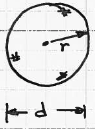
\includegraphics[width=1in]{drop.png} 
%   \caption{}
%   \label{fig:drop}
%\end{figure}

%Determine:
%\begin{enumerate}
%\item The gage pressure of the water in the drop.
%\end{enumerate}
%\noindent\rule{\linewidth}{0.4pt}
\clearpage
%\noindent\rule{\linewidth}{0.4pt}
\item A large atmospheric tank used for quenching rocket motors is filled with a Class A auto-foaming fire supressant liquid (specific weight 7595 N/m$^3$).  The supressant is restrained by a circular gate as shown.\footnote{When a rocket motor quench is needed, the gate is lifted and the suppressant rapidly flows over the test area.}  

\begin{figure}[h!] %  figure placement: here, top, bottom, or page
   \centering
   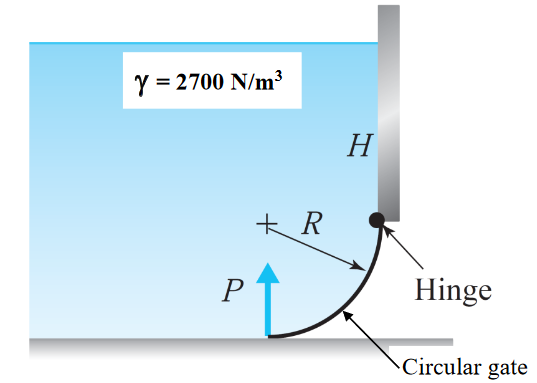
\includegraphics[width=3in]{circlegate.png} 
   \caption{}
   \label{fig:circlegate}
\end{figure}

The dimensions of interest are: R = 1.5 m, H = 6 m, Gate width (into the plane of the image) b = 3 m.

Determine:
\begin{enumerate}
\item The liquid pressure at the hinge.
\item The liquid pressure at the bottom of the gate
\item The horizontal and vertical force of the liquid acting on the circular gate
\end{enumerate}
\noindent\rule{\linewidth}{0.4pt}
%\clearpage
%~\newline
\end{enumerate}
%%%%%%%%%%%%%%%%%%%%%%%%%%%%%%%%%%%%%%%%%%%%%%%%%%%%%%%%%%%%%%%%%%%%%%%%%%%%%%%%%%%%
\bibliographystyle{chicago}	         % (uses file "chicago.bst")
\end{document}


